\subsection{座標系と回転}

本章のここまででは、差動二輪ロボットのオドメトリが車輪すべりでずれること、IMU のジャイロ積分がバイアスで漂うこと、加速度計の重力方向がロール・ピッチを低周波側から拘束することを見た。相補フィルタは速いジャイロと遅い重力測定を混ぜ、Kalman フィルタと EKF は残った不確かさを共分散と線形化で扱い、ESKF は名目状態と小さな誤差状態を分けて姿勢の制約を壊さないようにした。ここで次の制限が現れる。平面の向き $\theta$ だけなら角度の足し算で済むが、小型マルチコプタ、手先姿勢、カメラと IMU の外部パラメータのように三次元姿勢を扱うと、どの座標系の成分か、どの姿勢表現を内部状態に使うか、どの接空間で誤差を線形化するかを同時に決めなければならない。

空間を動く対象では、同じ物理ベクトルをどの座標系の成分として表しているかを明確にしなければならない。たとえば慣性座標系を $\{I\}$、対象に固定した機体座標系を $\{B\}$ とする。位置、速度、力、角速度はすべてベクトルであるが、成分表示は座標系に依存する。慣性座標系で表した位置を $p^I$ [m]、機体座標系で表した力を $f^B$ [N] のように書く。右肩の記号は、量そのものの種類ではなく、成分を読んでいる座標系を示す。

この区別を無視すると、力学式そのものが別の物理を表してしまう。質量 $1.2$ [kg] の小型マルチコプタがロール角 $30^\circ$ の姿勢で機体上向き推力
\begin{equation}
  f^B=
  \begin{bmatrix}
    0\\0\\12
  \end{bmatrix}\ \mathrm{N}
\end{equation}
を出している場面を考える。推力を慣性座標系の力としてそのまま足すと、水平方向の加速度は 0 と計算される。しかし実際には推力方向も機体と一緒に傾いており、後で定義する変換を用いると慣性座標系の力はおよそ
\begin{equation}
  R^I_B f^B\simeq
  \begin{bmatrix}
    0\\-6.0\\10.4
  \end{bmatrix}\ \mathrm{N}
\end{equation}
である。横向き成分 $-6.0$ [N] は加速度にして約 $-5.0$ [m/s$^2$] であり、これを無視したモデルでは姿勢制御、軌道予測、NMPC の制約評価、IMU と推力モデルを使う推定が同じ向きにずれる。座標変換は表記の好みではなく、力、速度、センサ値を同じ式に入れるための物理的な前処理である。

\subsubsection{座標成分と座標変換}

座標系 $\{A\}$ と $\{B\}$ がどちらも右手系の直交基底を持つとする。$\{B\}$ の各基底ベクトルを $\{A\}$ の成分で並べた行列を
\begin{equation}
  R^A_B=
  \begin{bmatrix}
    \left(e^B_1\right)^A&
    \left(e^B_2\right)^A&
    \left(e^B_3\right)^A
  \end{bmatrix}
\end{equation}
と定義する。この行列は、$\{B\}$ 成分で書いた自由ベクトル $v^B$ を、同じ幾何ベクトルの $\{A\}$ 成分へ変換する。
\begin{equation}
  v^A=R^A_B v^B.
\end{equation}
点の位置には、原点のずれも入る。$\{B\}$ の原点が $\{A\}$ で $r^A_{AB}$ [m] にあるなら、$\{B\}$ 成分で表した点 $p^B$ の $\{A\}$ 成分は
\begin{equation}
  p^A=r^A_{AB}+R^A_B p^B
\end{equation}
である。力や速度のような自由ベクトルでは平行移動 $r^A_{AB}$ は現れないが、位置点では回転と平行移動を区別する必要がある。

\begin{figure}[tb]
\centering
\setlength{\unitlength}{0.82mm}
\begin{picture}(135,72)
  \small
  \thinlines
  \put(20,15){\vector(1,0){34}}
  \put(20,15){\vector(0,1){30}}
  \put(20,15){\vector(-1,-1){12}}
  \put(55,13){\makebox(0,0)[t]{$x_A$}}
  \put(17,47){\makebox(0,0)[r]{$y_A$}}
  \put(7,1){\makebox(0,0)[t]{$z_A$}}
  \put(17,12){\makebox(0,0)[r]{$\{A\}$}}
  \put(68,39){\vector(1,1){18}}
  \put(68,39){\vector(-1,2){13}}
  \put(68,39){\vector(1,0){24}}
  \put(88,58){\makebox(0,0)[l]{$x_B$}}
  \put(54,66){\makebox(0,0)[r]{$y_B$}}
  \put(94,37){\makebox(0,0)[l]{$z_B$}}
  \put(66,35){\makebox(0,0)[r]{$\{B\}$}}
  \thicklines
  \put(20,15){\vector(2,1){48}}
  \put(43,31){\makebox(0,0)[b]{$r^A_{AB}$}}
  \put(68,39){\vector(1,1){24}}
  \put(82,54){\makebox(0,0)[l]{$R^A_Bp^B$}}
  \put(20,15){\vector(3,2){72}}
  \put(62,58){\makebox(0,0)[l]{$p^A$}}
  \put(94,63){\circle*{2}}
  \put(98,63){\makebox(0,0)[l]{$P$}}
  \put(18,7){\makebox(100,0)[l]{$p^A=r^A_{AB}+R^A_Bp^B$}}
\end{picture}
\caption{座標系の原点移動と回転を含む点の座標変換}
\label{fig:coordinate-frame-transform}
\end{figure}

図\ref{fig:coordinate-frame-transform} は、点 $P$ の同じ幾何的位置を、原点移動 $r^A_{AB}$ と回転 $R^A_B$ によって座標系 $\{A\}$ の成分へ変換する関係を示している。自由ベクトルと位置点を区別するため、位置点では回転項に加えて原点の平行移動が必要になる。

以降では、$R^A_B$ と $T^A_B$ は常に「$\{B\}$ 成分で書いた量を $\{A\}$ 成分へ変換する」写像を表し、列ベクトルの左から作用させる。上付きの座標系が出力成分、下付きの座標系が入力成分である。この向きを固定しておくと、$R^A_BR^B_C$ のような積では中央の座標系 $\{B\}$ が消え、$\{C\}$ 成分から $\{A\}$ 成分への変換になることを添字から判定できる。

\subsubsection{二次元と三次元の回転行列}

平面で角度 $\theta$ だけ反時計回りに向きを変える回転行列は
\begin{equation}
  R_2(\theta)=
  \begin{bmatrix}
    \cos\theta&-\sin\theta\\
    \sin\theta& \cos\theta
  \end{bmatrix}
\end{equation}
である。第一列は、回転後の $x$ 軸の単位ベクトルをもとの座標系で表した成分であり、第二列は回転後の $y$ 軸の単位ベクトルである。三次元では、右手系の規約に従って各軸まわりの基本回転を
\begin{align}
  R_x(\phi)&=
  \begin{bmatrix}
    1&0&0\\
    0&\cos\phi&-\sin\phi\\
    0&\sin\phi& \cos\phi
  \end{bmatrix},\\
  R_y(\theta)&=
  \begin{bmatrix}
    \cos\theta&0&\sin\theta\\
    0&1&0\\
    -\sin\theta&0&\cos\theta
  \end{bmatrix},\\
  R_z(\psi)&=
  \begin{bmatrix}
    \cos\psi&-\sin\psi&0\\
    \sin\psi& \cos\psi&0\\
    0&0&1
  \end{bmatrix}
\end{align}
と置く。ロール $\phi$、ピッチ $\theta$、ヨー $\psi$ の ZYX オイラー角では、機体座標系から慣性座標系への姿勢を
\begin{equation}
  R^I_B=R_z(\psi)R_y(\theta)R_x(\phi)
\end{equation}
のように表す。行列積の順序は回転順序を含んでいるため、同じ三つの角でも順序を変えれば一般に別の姿勢になる。

\subsubsection{オイラー角の回転順序とジンバルロック}

三次元姿勢は 3 個の自由度を持つため、3 個の角度で表すことは自然な表現である。しかし、どの軸まわりに、どの順序で回転するかを指定しない限り、角度の組は姿勢を定めない。一般に軸列 $a,b,c\in\{x,y,z\}$ を決めると
\begin{equation}
  R_{abc}(\alpha,\beta,\gamma)
  =R_a(\alpha)R_b(\beta)R_c(\gamma)
\end{equation}
のような回転列を定義できる。列ベクトルに右から作用させる約束では、右端の $R_c(\gamma)$ が最初に作用する。よく用いられる ZYX 表現は
\begin{equation}
  R^I_B=R_z(\psi)R_y(\theta)R_x(\phi)
\end{equation}
であり、$\phi$ をロール角、$\theta$ をピッチ角、$\psi$ をヨー角と呼ぶ。これは航空機や移動体の姿勢表示では解釈しやすいが、制御器や推定器の内部状態として常に安全な座標とは限らない。

回転行列の積は一般には交換できない。たとえば
\begin{equation}
  R_z(\pi/2)R_x(\pi/2)
  \begin{bmatrix}0\\0\\1\end{bmatrix}
  =
  \begin{bmatrix}1\\0\\0\end{bmatrix},
  \qquad
  R_x(\pi/2)R_z(\pi/2)
  \begin{bmatrix}0\\0\\1\end{bmatrix}
  =
  \begin{bmatrix}0\\-1\\0\end{bmatrix}
\end{equation}
である。同じ $90^\circ$ の $x$ 軸回転と $z$ 軸回転を使っても、順序が変われば最終的なベクトルは変わる。したがって、オイラー角を記録するときは、数値だけでなく ZYX、XYZ、ZXZ などの回転順序と、能動回転か受動変換かを同時に明記する必要がある。

ZYX オイラー角の時間微分と機体系角速度 $\omega^B=[p\ q\ r]^\T$ [rad/s] の関係は
\begin{equation}
  \omega^B=
  \begin{bmatrix}
    1&0&-\sin\theta\\
    0&\cos\phi&\sin\phi\cos\theta\\
    0&-\sin\phi&\cos\phi\cos\theta
  \end{bmatrix}
  \begin{bmatrix}
    \dot{\phi}\\ \dot{\theta}\\ \dot{\psi}
  \end{bmatrix}
\end{equation}
である。この式をオイラー角速度について解くと
\begin{equation}
  \begin{bmatrix}
    \dot{\phi}\\ \dot{\theta}\\ \dot{\psi}
  \end{bmatrix}
  =
  \begin{bmatrix}
    1&\sin\phi\tan\theta&\cos\phi\tan\theta\\
    0&\cos\phi&-\sin\phi\\
    0&\sin\phi/\cos\theta&\cos\phi/\cos\theta
  \end{bmatrix}
  \begin{bmatrix}
    p\\ q\\ r
  \end{bmatrix}
\end{equation}
となる。右辺には $1/\cos\theta$ と $\tan\theta$ が現れるので、$\cos\theta=0$、すなわち $\theta=\pm\pi/2$ [rad] では写像が特異になる。この特異性をジンバルロックという。

ジンバルロックは、実際の剛体が回転できなくなる現象ではなく、選んだ座標表示が一意性を失う現象である。たとえば $\theta=\pi/2$ では
\begin{equation}
  R_z(\psi)R_y(\pi/2)R_x(\phi)
  =
  \begin{bmatrix}
    0&\sin(\phi-\psi)&\cos(\phi-\psi)\\
    0&\cos(\phi-\psi)&-\sin(\phi-\psi)\\
    -1&0&0
  \end{bmatrix}
\end{equation}
となり、姿勢は $\phi-\psi$ だけに依存する。したがって、$\phi$ と $\psi$ を別々に変えても同じ姿勢を表す組が存在する。この近くでは、わずかな角速度をオイラー角速度へ換算するだけで非常に大きな $\dot{\phi}$ や $\dot{\psi}$ が計算されることがあり、数値積分、姿勢推定のヤコビアン、姿勢制御の誤差計算を不安定にする。

この悪条件性は数値で見るとさらに明確である。$\phi=0$、$p=q=0$、機体系の $z$ 軸角速度 $r=0.10$ [rad/s] だけがある場合、逆変換式から
\begin{equation}
  \dot{\phi}=r\tan\theta,\qquad
  \dot{\psi}=\frac{r}{\cos\theta}
\end{equation}
となる。
\begin{center}
\begin{tabular}{c|c|c|c}
$\theta$ & $|\cos\theta|$ & $1/|\cos\theta|$ & $\dot{\psi}$ [rad/s]\\
\hline
$0^\circ$ & $1.000$ & $1.0$ & $0.10$\\
$60^\circ$ & $0.500$ & $2.0$ & $0.20$\\
$80^\circ$ & $0.174$ & $5.8$ & $0.58$\\
$89^\circ$ & $0.017$ & $57.3$ & $5.73$
\end{tabular}
\end{center}
機体の実角速度は同じ $0.10$ [rad/s] でも、ピッチ角が $89^\circ$ に近づくとヨー角速度の表示は約 $57$ 倍に増幅される。制御器がオイラー角速度を直接指令値として飽和判定すると、実際の剛体運動ではなく座標表示の悪条件性によって大きな角速度指令や共分散増大が生じる。

オイラー角は、人が理解する表示、操作量のログ、ピッチ角やヨー角を直接制限する制約条件には有用である。一方、全姿勢を連続的に推定・制御する内部表現としては、特異点を避けるために回転行列、単位四元数、または $\SO(3)$ 上の指数写像と対数写像を併用する。

\subsubsection{直交条件と特殊直交群}

回転は長さと内積を保つ変換である。任意のベクトル $v$ に対して長さが変わらないなら
\begin{equation}
  \norm{Rv}^2=(Rv)^\T(Rv)=v^\T R^\T R v
  =v^\T v
\end{equation}
がすべての $v$ で成り立つので、
\begin{equation}
  R^\T R=I
\end{equation}
でなければならない。この条件は、$R$ の列ベクトルが互いに直交し、すべて長さ 1 であることを意味する。したがって逆行列は
\begin{equation}
  R^{-1}=R^\T
\end{equation}
であり、座標変換を戻す計算は転置で済む。

行列式を取ると
\begin{equation}
  \det(R^\T R)=\det I
  \quad\Longrightarrow\quad
  (\det R)^2=1
\end{equation}
なので、直交行列では $\det R=1$ または $\det R=-1$ である。$\det R=-1$ は鏡映を含む向き反転であり、右手系を左手系へ移す。剛体の姿勢を表す純粋な回転では向きを反転しないため、$\det R=1$ を要求する。

\begin{definition}[特殊直交群]
三次元の純粋な回転行列全体の集合
\begin{equation}
  \SO(3)=\{R\in\R^{3\times3}\mid R^\T R=I,\ \det R=1\}
\end{equation}
を三次元特殊直交群という。$R_1,R_2\in\SO(3)$ なら $R_1R_2\in\SO(3)$、また $R^{-1}=R^\T\in\SO(3)$ であるため、回転の合成と逆変換は同じ集合の中に残る。
\end{definition}

$\SO(3)$ の条件は、姿勢行列を単なる 9 成分の配列として扱わないための制約である。たとえば重力方向 $g^I$ を機体系へ変換するとき、$R^B_I=(R^I_B)^\T$ が直交性を失っていると、長さが保たれず、加速度計が観測した重力の大きさまで変化したと解釈される。姿勢推定や姿勢制御では、この偽の変化を実加速度や外乱トルクとして誤って吸収しないように、名目姿勢を常に $\SO(3)$ 上に残す。

\subsubsection{同次変換と特殊ユークリッド群}

剛体の配置は、向きだけでなく原点の位置も含めて定める。座標系 $\{B\}$ が剛体に固定され、座標系 $\{A\}$ が基準座標系であるとする。$\{B\}$ から $\{A\}$ への姿勢を $R^A_B\in\SO(3)$、$\{B\}$ の原点の $\{A\}$ 成分を $r^A_{AB}\in\R^3$ [m] と書く。この組
\begin{equation}
  (R^A_B,r^A_{AB})
\end{equation}
を、$\{B\}$ の $\{A\}$ に対する剛体配置または pose という。一般記号では pose を $(R,p)$ と略記し、$R\in\SO(3)$、$p\in\R^3$ [m] を仮定する。

回転と平行移動を一つの行列積で扱うため、点 $p^B\in\R^3$ [m] に同次座標
\begin{equation}
  \bar{p}^B=
  \begin{bmatrix}
    p^B\\1
  \end{bmatrix}
\end{equation}
を対応させる。pose $(R^A_B,r^A_{AB})$ の同次変換行列を
\begin{equation}
  T^A_B=
  \begin{bmatrix}
    R^A_B&r^A_{AB}\\
    0_{1\times3}&1
  \end{bmatrix}
\end{equation}
と定義すると、点の座標変換は
\begin{equation}
  \bar{p}^A=T^A_B\bar{p}^B
  =
  \begin{bmatrix}
    R^A_Bp^B+r^A_{AB}\\
    1
  \end{bmatrix}
\end{equation}
である。最後の成分を 1 にしたことにより、回転と平行移動が同じ行列積に入る。一方、力、速度、角速度のような自由ベクトルには原点の平行移動は作用しないため、同次座標で表すなら最後の成分を 0 として
\begin{equation}
  \begin{bmatrix}
    v^A\\0
  \end{bmatrix}
  =
  T^A_B
  \begin{bmatrix}
    v^B\\0
  \end{bmatrix}
  =
  \begin{bmatrix}
    R^A_Bv^B\\0
  \end{bmatrix}
\end{equation}
と表す。

\begin{definition}[特殊ユークリッド群]
三次元剛体配置を表す同次変換行列全体の集合
\begin{equation}
  \operatorname{SE}(3)
  =
  \left\{
  \begin{bmatrix}
    R&p\\
    0_{1\times3}&1
  \end{bmatrix}
  \middle|
  R\in\SO(3),\ p\in\R^3
  \right\}
\end{equation}
を三次元特殊ユークリッド群という。これは回転と平行移動の合成を表す群であり、剛体運動の座標変換は $\operatorname{SE}(3)$ の元として扱える。
\end{definition}

座標系が $\{A\}$、$\{B\}$、$\{C\}$ と連なるとき、$\{C\}$ から $\{A\}$ への pose は同次変換の積で
\begin{equation}
  T^A_C=T^A_BT^B_C
\end{equation}
と得られる。成分を展開すると
\begin{align}
  T^A_BT^B_C
  &=
  \begin{bmatrix}
    R^A_B&r^A_{AB}\\
    0&1
  \end{bmatrix}
  \begin{bmatrix}
    R^B_C&r^B_{BC}\\
    0&1
  \end{bmatrix}\\
  &=
  \begin{bmatrix}
    R^A_BR^B_C&r^A_{AB}+R^A_Br^B_{BC}\\
    0&1
  \end{bmatrix}.
\end{align}
したがって
\begin{equation}
  R^A_C=R^A_BR^B_C,\qquad
  r^A_{AC}=r^A_{AB}+R^A_Br^B_{BC}
\end{equation}
である。第二式は、$\{A\}$ から $\{B\}$ 原点まで進み、さらに $\{B\}$ 成分で与えられた $\{C\}$ 原点の位置を $\{A\}$ 成分へ変換して加える、という合成規則を表している。この規約では、$\hat{T}^A_B$ に機体系側で表した小さな pose 増分を入れるなら右から掛け、基準座標系側で表した小さな pose 増分を入れるなら左から掛ける。右掛けと左掛けは同じ補正量の別表記ではなく、どの座標系で誤差を表しているかを決める操作である。

逆変換も同じ集合に残る。$T^A_B$ の逆は
\begin{equation}
  T^B_A=(T^A_B)^{-1}
  =
  \begin{bmatrix}
    (R^A_B)^\T&-(R^A_B)^\T r^A_{AB}\\
    0&1
  \end{bmatrix}
\end{equation}
であり、対応する pose の逆は
\begin{equation}
  (R,p)^{-1}=(R^\T,-R^\T p)
\end{equation}
である。実際に積を取ると
\begin{align}
  T^B_AT^A_B
  &=
  \begin{bmatrix}
    (R^A_B)^\T&-(R^A_B)^\T r^A_{AB}\\
    0&1
  \end{bmatrix}
  \begin{bmatrix}
    R^A_B&r^A_{AB}\\
    0&1
  \end{bmatrix}\\
  &=
  \begin{bmatrix}
    I&0\\
    0&1
  \end{bmatrix}
\end{align}
となる。

剛体の状態方程式では、配置 $T^I_B=(R^I_B,r^I_{IB})$ が位置と姿勢の幾何学的な部分を担い、速度 $v^I$ [m/s] と角速度 $\omega^B$ [rad/s] はその時間変化を表す接ベクトルとして加わる。したがって、剛体状態は
\begin{equation}
  x=(T^I_B,\ v^I,\ \omega^B)
\end{equation}
または、$p^I=r^I_{IB}$ とおいて同じ内容を成分に分けて
\begin{equation}
  x=(p^I,\ v^I,\ R^I_B,\ \omega^B)
\end{equation}
と書ける。制御や推定で pose 誤差を作るときは、位置と回転を成分ごとに単純に引くのではなく、相対変換
\begin{equation}
  \tilde{T}=(\hat{T}^A_B)^{-1}T^A_B
  =
  \begin{bmatrix}
    (\hat{R}^A_B)^\T R^A_B&
    (\hat{R}^A_B)^\T(r^A_{AB}-\hat{r}^A_{AB})\\
    0&1
  \end{bmatrix}
\end{equation}
を構成する。ここから
\begin{equation}
  e_p=(\hat{R}^A_B)^\T(r^A_{AB}-\hat{r}^A_{AB}),\qquad
  e_R=\operatorname{Log}\{(\hat{R}^A_B)^\T R^A_B\}^\vee
\end{equation}
のように、位置誤差と小角度姿勢誤差を推定座標系側のベクトルとして取り出せる。ここで $\operatorname{Log}$ は後で形式的に定義する回転群の対数写像であり、$e_p$ の単位は [m]、$e_R$ の単位は [rad] である。この表現は、姿勢制御、後で扱う姿勢推定、NMPC で、名目 pose は $\operatorname{SE}(3)$ 上に保ち、誤差だけを局所的なベクトルとして線形化するための基礎になる。

\subsubsection{能動変換と受動変換}

回転行列には二つの解釈がある。受動的な解釈では、幾何ベクトルは固定したまま、成分表示に用いる座標系だけを変える。たとえば
\begin{equation}
  v^A=R^A_B v^B,
  \qquad
  v^B=(R^A_B)^\T v^A
\end{equation}
は、同じベクトルを $\{B\}$ 成分と $\{A\}$ 成分で読み替えている。一方、能動的な解釈では、同じ座標系の中でベクトルそのものを回転させる。
\begin{equation}
  v_{\mathrm{rot}}^A=R v^A
\end{equation}
は、$\{A\}$ 成分で書いたベクトル $v^A$ を物理的に回転させた新しいベクトルの $\{A\}$ 成分である。数式の形は似ているが、受動変換では「同じ量の座標成分の変更」、能動変換では「別の量への回転」を表す。この区別を曖昧にすると、センサが測った加速度、機体座標系の推力、慣性座標系の速度を同じ式に混ぜてしまう。

座標系が $\{A\}$、$\{B\}$、$\{C\}$ と連なる場合、$\{C\}$ 成分から $\{A\}$ 成分への変換は
\begin{equation}
  R^A_C=R^A_B R^B_C
\end{equation}
である。実際、
\begin{equation}
  v^A=R^A_B v^B=R^A_B R^B_C v^C
\end{equation}
なので、右から順に座標系をたどる。逆向きの変換は
\begin{equation}
  R^B_A=(R^A_B)^\T
\end{equation}
であり、位置点の逆変換は
\begin{equation}
  p^B=(R^A_B)^\T\left(p^A-r^A_{AB}\right)
\end{equation}
となる。

\begin{example}[平面移動体の速度変換]
平面上の移動体が慣性座標系に対してヨー角 $\psi=\pi/6$ [rad] を持ち、機体座標系で前方速度
\begin{equation}
  v^B=
  \begin{bmatrix}2\\0\end{bmatrix}\ \mathrm{m/s}
\end{equation}
を持つとする。慣性座標系での速度は
\begin{equation}
  v^I=R_2(\psi)v^B
  =
  \begin{bmatrix}
    \cos(\pi/6)&-\sin(\pi/6)\\
    \sin(\pi/6)& \cos(\pi/6)
  \end{bmatrix}
  \begin{bmatrix}2\\0\end{bmatrix}
  =
  \begin{bmatrix}\sqrt{3}\\1\end{bmatrix}\ \mathrm{m/s}
\end{equation}
である。位置状態を慣性座標系で $p^I=[x\ y]^\T$ と置くなら、状態方程式には
\begin{equation}
  \dot{p}^I=v^I=R_2(\psi)v^B
\end{equation}
を使う。ここで $\dot{p}^I=v^B$ と書くと、機体前方成分を慣性座標系の $x$ 方向成分として扱うことになり、向きが変わる運動を正しく表せない。
\end{example}

\subsubsection{状態変数と力学における役割}

座標変換は記号上の整理ではなく、状態方程式の構造を決める。剛体の状態を、慣性座標系で表した位置 $p^I$ [m]、速度 $v^I$ [m/s]、機体から慣性系への姿勢 $R^I_B\in\SO(3)$、機体系角速度 $\omega^B$ [rad/s] で
\begin{equation}
  x=\left(p^I,\ v^I,\ R^I_B,\ \omega^B\right)
\end{equation}
と選ぶ。このとき機体系で生じる合力 $f^B$ を並進運動へ入れるには
\begin{equation}
  m\dot{v}^I=mg^I+R^I_B f^B
\end{equation}
のように慣性座標系へ変換しなければならない。また、機体系角速度を使う姿勢運動は
\begin{equation}
  \dot{R}^I_B=R^I_B[\omega^B]_\times
\end{equation}
で書ける。ただし
\begin{equation}
  [\omega]_\times=
  \begin{bmatrix}
    0&-\omega_3&\omega_2\\
    \omega_3&0&-\omega_1\\
    -\omega_2&\omega_1&0
  \end{bmatrix},
  \qquad
  [\omega]_\times a=\omega\times a
\end{equation}
である。

$R^I_B$ は $3\times3$ 行列なので 9 個の成分を持つが、$R^\T R=I$ と $\det R=1$ の制約により独立な姿勢自由度は 3 である。したがって、数値積分や姿勢推定で行列成分に任意の補正を足すと、一般には $\SO(3)$ から外れる。姿勢を状態に含む制御と推定では、回転そのものは $\SO(3)$ 上に保ち、小さな誤差だけを三次元ベクトルとして扱う設計が必要になる。この事実が、四元数、指数写像、局所誤差を用いる姿勢推定へつながる。

\subsubsection{単位四元数による姿勢表現}

四元数は、スカラー部 $q_0\in\R$ とベクトル部 $q_v\in\R^3$ を持つ 4 成分の量
\begin{equation}
  q=
  \begin{bmatrix}
    q_0\\ q_v
  \end{bmatrix}
\end{equation}
である。姿勢を表すときは単位制約
\begin{equation}
  \norm{q}=1
\end{equation}
を課す。単位軸 $a\in\R^3$、$\norm{a}=1$ のまわりに角度 $\theta$ [rad] だけ回転する姿勢は
\begin{equation}
  q=
  \begin{bmatrix}
    \cos(\theta/2)\\
    a\sin(\theta/2)
  \end{bmatrix}
\end{equation}
で表される。角度が半分で現れるため、$q$ と $-q$ は同じ回転を表す。この二重被覆は、姿勢ログや補間で符号が急に反転して現れる原因になるので、連続した時系列では隣り合う四元数の内積が負になったら片方の符号を反転する、という処理を入れることが多い。

四元数の積を
\begin{equation}
  q\otimes p
  =
  \begin{bmatrix}
    q_0p_0-q_v^\T p_v\\
    q_0p_v+p_0q_v+q_v\times p_v
  \end{bmatrix}
\end{equation}
で定義する。単位四元数の共役は
\begin{equation}
  q^*=
  \begin{bmatrix}
    q_0\\ -q_v
  \end{bmatrix}
\end{equation}
であり、$\norm{q}=1$ なら $q^{-1}=q^*$ である。$q^A_B$ を $\{B\}$ 成分から $\{A\}$ 成分への姿勢と対応させると、ベクトル $v^B$ の変換は純四元数 $[0\ (v^B)^\T]^\T$ を用いて
\begin{equation}
  \begin{bmatrix}
    0\\ v^A
  \end{bmatrix}
  =
  q^A_B\otimes
  \begin{bmatrix}
    0\\ v^B
  \end{bmatrix}
  \otimes(q^A_B)^*
\end{equation}
と書ける。

姿勢の合成は回転行列と同じ順序構造を持つ。座標系が $\{A\}$、$\{B\}$、$\{C\}$ と連なるなら
\begin{equation}
  q^A_C=q^A_B\otimes q^B_C
\end{equation}
である。たとえば $z$ 軸まわり $90^\circ$ の回転
\begin{equation}
  q_z=
  \begin{bmatrix}
    \sqrt{2}/2\\0\\0\\\sqrt{2}/2
  \end{bmatrix}
\end{equation}
と $x$ 軸まわり $90^\circ$ の回転
\begin{equation}
  q_x=
  \begin{bmatrix}
    \sqrt{2}/2\\\sqrt{2}/2\\0\\0
  \end{bmatrix}
\end{equation}
を行列積 $R_z(\pi/2)R_x(\pi/2)$ に対応する順序で合成すると
\begin{equation}
  q_z\otimes q_x
  =
  \begin{bmatrix}
    1/2\\1/2\\1/2\\1/2
  \end{bmatrix}
\end{equation}
となる。この結果は、対応する回転行列の積 $R_z(\pi/2)R_x(\pi/2)$ と同じ姿勢を表す。

\subsubsection{四元数運動学と数値更新}

角速度の成分をどの座標系で表すかにより、四元数運動学の積の向きが変わる。$q^I_B$ が機体系から慣性系への姿勢を表し、角速度を機体系成分 $\omega^B$ [rad/s] で与えるなら
\begin{equation}
  \dot{q}^I_B
  =
  \frac{1}{2}q^I_B\otimes
  \begin{bmatrix}
    0\\ \omega^B
  \end{bmatrix}
\end{equation}
である。角速度を慣性系成分 $\omega^I=R^I_B\omega^B$ で与えるなら
\begin{equation}
  \dot{q}^I_B
  =
  \frac{1}{2}
  \begin{bmatrix}
    0\\ \omega^I
  \end{bmatrix}
  \otimes q^I_B
\end{equation}
と書く。同じ物理角速度でも、成分表示を変えたなら四元数積の左右も変わる。

サンプリング周期 $\Delta t$ [s] が短く、区間内で角速度を一定とみなすと、回転ベクトル
\begin{equation}
  \Delta\theta=\omega^B\Delta t
\end{equation}
に対応する増分四元数
\begin{equation}
  \delta q=
  \begin{cases}
    \begin{bmatrix}
      \cos(\norm{\Delta\theta}/2)\\
      \dfrac{\Delta\theta}{\norm{\Delta\theta}}
      \sin(\norm{\Delta\theta}/2)
    \end{bmatrix},
    & \norm{\Delta\theta}>0,\\[3ex]
    \begin{bmatrix}
      1\\0\\0\\0
    \end{bmatrix},
    & \norm{\Delta\theta}=0
  \end{cases}
\end{equation}
を作り、
\begin{equation}
  q^I_{B,k+1}=q^I_{B,k}\otimes\delta q
\end{equation}
で更新する。数値丸めや近似により $\norm{q}$ が 1 からずれるため、実装では
\begin{equation}
  q^I_{B,k+1}\leftarrow
  \frac{q^I_{B,k+1}}{\norm{q^I_{B,k+1}}}
\end{equation}
と正規化する。ただし、正規化は単位制約を戻す処理であり、ジャイロバイアス、積分誤差、外乱トルクを消す処理ではない。これらはモデル化し、推定器または制御器で扱う必要がある。

正規化が必要になる理由は、一次近似の更新を数値評価すると分かる。初期値 $q=[1\ 0\ 0\ 0]^\T$、角速度の大きさ $\norm{\omega}=2$ [rad/s]、$\Delta t=0.01$ [s] とし、指数写像ではなく
\begin{equation}
  q_{k+1}\simeq q_k+\frac{1}{2}q_k\otimes
  \begin{bmatrix}
    0\\ \omega
  \end{bmatrix}\Delta t
\end{equation}
で更新すると、1 ステップ後のノルムは
\begin{equation}
  \sqrt{1+(0.5\norm{\omega}\Delta t)^2}
  =
  \sqrt{1+0.01^2}
  \simeq 1.00005
\end{equation}
になる。このずれは小さいが、同じ近似を 1000 ステップ続けるとノルムは約 $1.051$ まで増える。単位四元数から回転行列を作る式は $\norm{q}=1$ を前提にしているため、このずれを放置すると、回転の合成が長さを保つという $\SO(3)$ の性質まで壊れる。

\subsubsection{SO(3) の指数写像と対数写像}

四元数は特異点を避ける実用的な姿勢表現であるが、姿勢誤差を最小の 3 成分で扱うには $\SO(3)$ の接空間を使うと整理しやすい。姿勢そのものを 3 成分で全域表示しようとするとオイラー角の特異点に直面するが、ある名目姿勢の近くの小さな差だけなら、接空間の 3 成分で十分に表せる。ベクトル $\varphi\in\R^3$ から歪対称行列を作る写像を
\begin{equation}
  \widehat{\varphi}=[\varphi]_\times
\end{equation}
と書き、その逆を $(\cdot)^\vee$ と書く。$\theta=\norm{\varphi}$ とすると、指数写像は Rodrigues の公式
\begin{equation}
  \operatorname{Exp}(\widehat{\varphi})
  =
  I
  +\frac{\sin\theta}{\theta}\widehat{\varphi}
  +\frac{1-\cos\theta}{\theta^2}\widehat{\varphi}^2
\end{equation}
で与えられる。$\varphi$ は回転軸と回転角を一つにまとめた回転ベクトルであり、$\theta$ が回転角、$\varphi/\theta$ が回転軸である。$\theta$ が小さいときは
\begin{equation}
  \operatorname{Exp}(\widehat{\varphi})
  \simeq I+\widehat{\varphi}
\end{equation}
であり、これは小角度近似そのものである。

逆に、$R\in\SO(3)$ から回転ベクトルを取り出す写像を対数写像という。$0<\theta<\pi$ で
\begin{equation}
  \theta=
  \cos^{-1}\left(\frac{\tr R-1}{2}\right)
\end{equation}
と置けば
\begin{equation}
  \operatorname{Log}(R)
  =
  \frac{\theta}{2\sin\theta}(R-R^\T),
  \qquad
  \operatorname{Log}(R)^\vee
  =
  \frac{\theta}{2\sin\theta}(R-R^\T)^\vee
\end{equation}
である。$\theta$ が 0 に近いときは数値的に $0/0$ に近づくため、級数近似を使う。$\theta$ が $\pi$ に近いときは回転軸の符号選択が不安定になりやすい。したがって、対数写像は局所誤差には非常に有用だが、$180^\circ$ 近傍の大誤差を単純な線形誤差として扱うことは避ける。NMPC の線形化点や姿勢推定の名目姿勢は、この「対数写像が小さい範囲」に予測と補正を留めるための基準姿勢として働く。

\begin{example}[小さな姿勢誤差の対数写像]
推定姿勢 $\hat{R}$ と真の姿勢 $R$ の差が、機体系の $z$ 軸まわり $0.02$ [rad] の小回転だけであるとする。このとき
\begin{equation}
  \tilde{R}=\hat{R}^\T R=R_z(0.02)
\end{equation}
であり、
\begin{equation}
  \operatorname{Log}(\tilde{R})^\vee
  \simeq
  \begin{bmatrix}
    0\\0\\0.02
  \end{bmatrix}
\end{equation}
となる。誤差をオイラー角差として引き算すると、基準姿勢や回転順序によって値が変わるが、$\hat{R}^\T R$ の対数写像は「推定姿勢から真の姿勢へ戻す小回転」を直接表す。
\end{example}

\subsubsection{小角度誤差と姿勢推定・制御}

姿勢推定では、名目姿勢 $\hat{R}\in\SO(3)$ と小さな誤差 $\delta\theta\in\R^3$ を分けて
\begin{equation}
  R=\hat{R}\operatorname{Exp}(\widehat{\delta\theta})
\end{equation}
のように表す。これは右側から小回転を掛ける規約であり、$\delta\theta$ は推定された機体系側の局所誤差成分である。左側から小回転を掛ける規約を選ぶ場合は、誤差成分が慣性座標系側で表されるため、ヤコビアンと共分散の座標系も合わせて変えなければならない。右辺の $\delta\theta$ は、$\hat{R}$ そのものへ直接足す量ではなく、接空間で表した小回転である。誤差行列
\begin{equation}
  \tilde{R}=\hat{R}^\T R
\end{equation}
を使えば
\begin{equation}
  \delta\theta=\operatorname{Log}(\tilde{R})^\vee
\end{equation}
であり、小角度では
\begin{equation}
  \tilde{R}\simeq I+\widehat{\delta\theta},
  \qquad
  \delta\theta
  \simeq
  \frac{1}{2}(\tilde{R}-\tilde{R}^\T)^\vee
\end{equation}
となる。四元数で同じ誤差を表すなら、$\delta\theta\ne0$ で
\begin{equation}
  \delta q
  =
  \begin{bmatrix}
    \cos(\norm{\delta\theta}/2)\\
    \dfrac{\delta\theta}{\norm{\delta\theta}}
    \sin(\norm{\delta\theta}/2)
  \end{bmatrix}
  \simeq
  \begin{bmatrix}
    1\\ \delta\theta/2
  \end{bmatrix}
\end{equation}
である。これは後で扱う、名目姿勢と局所誤差を分ける更新式の基礎になる。

\begin{figure}[tb]
\centering
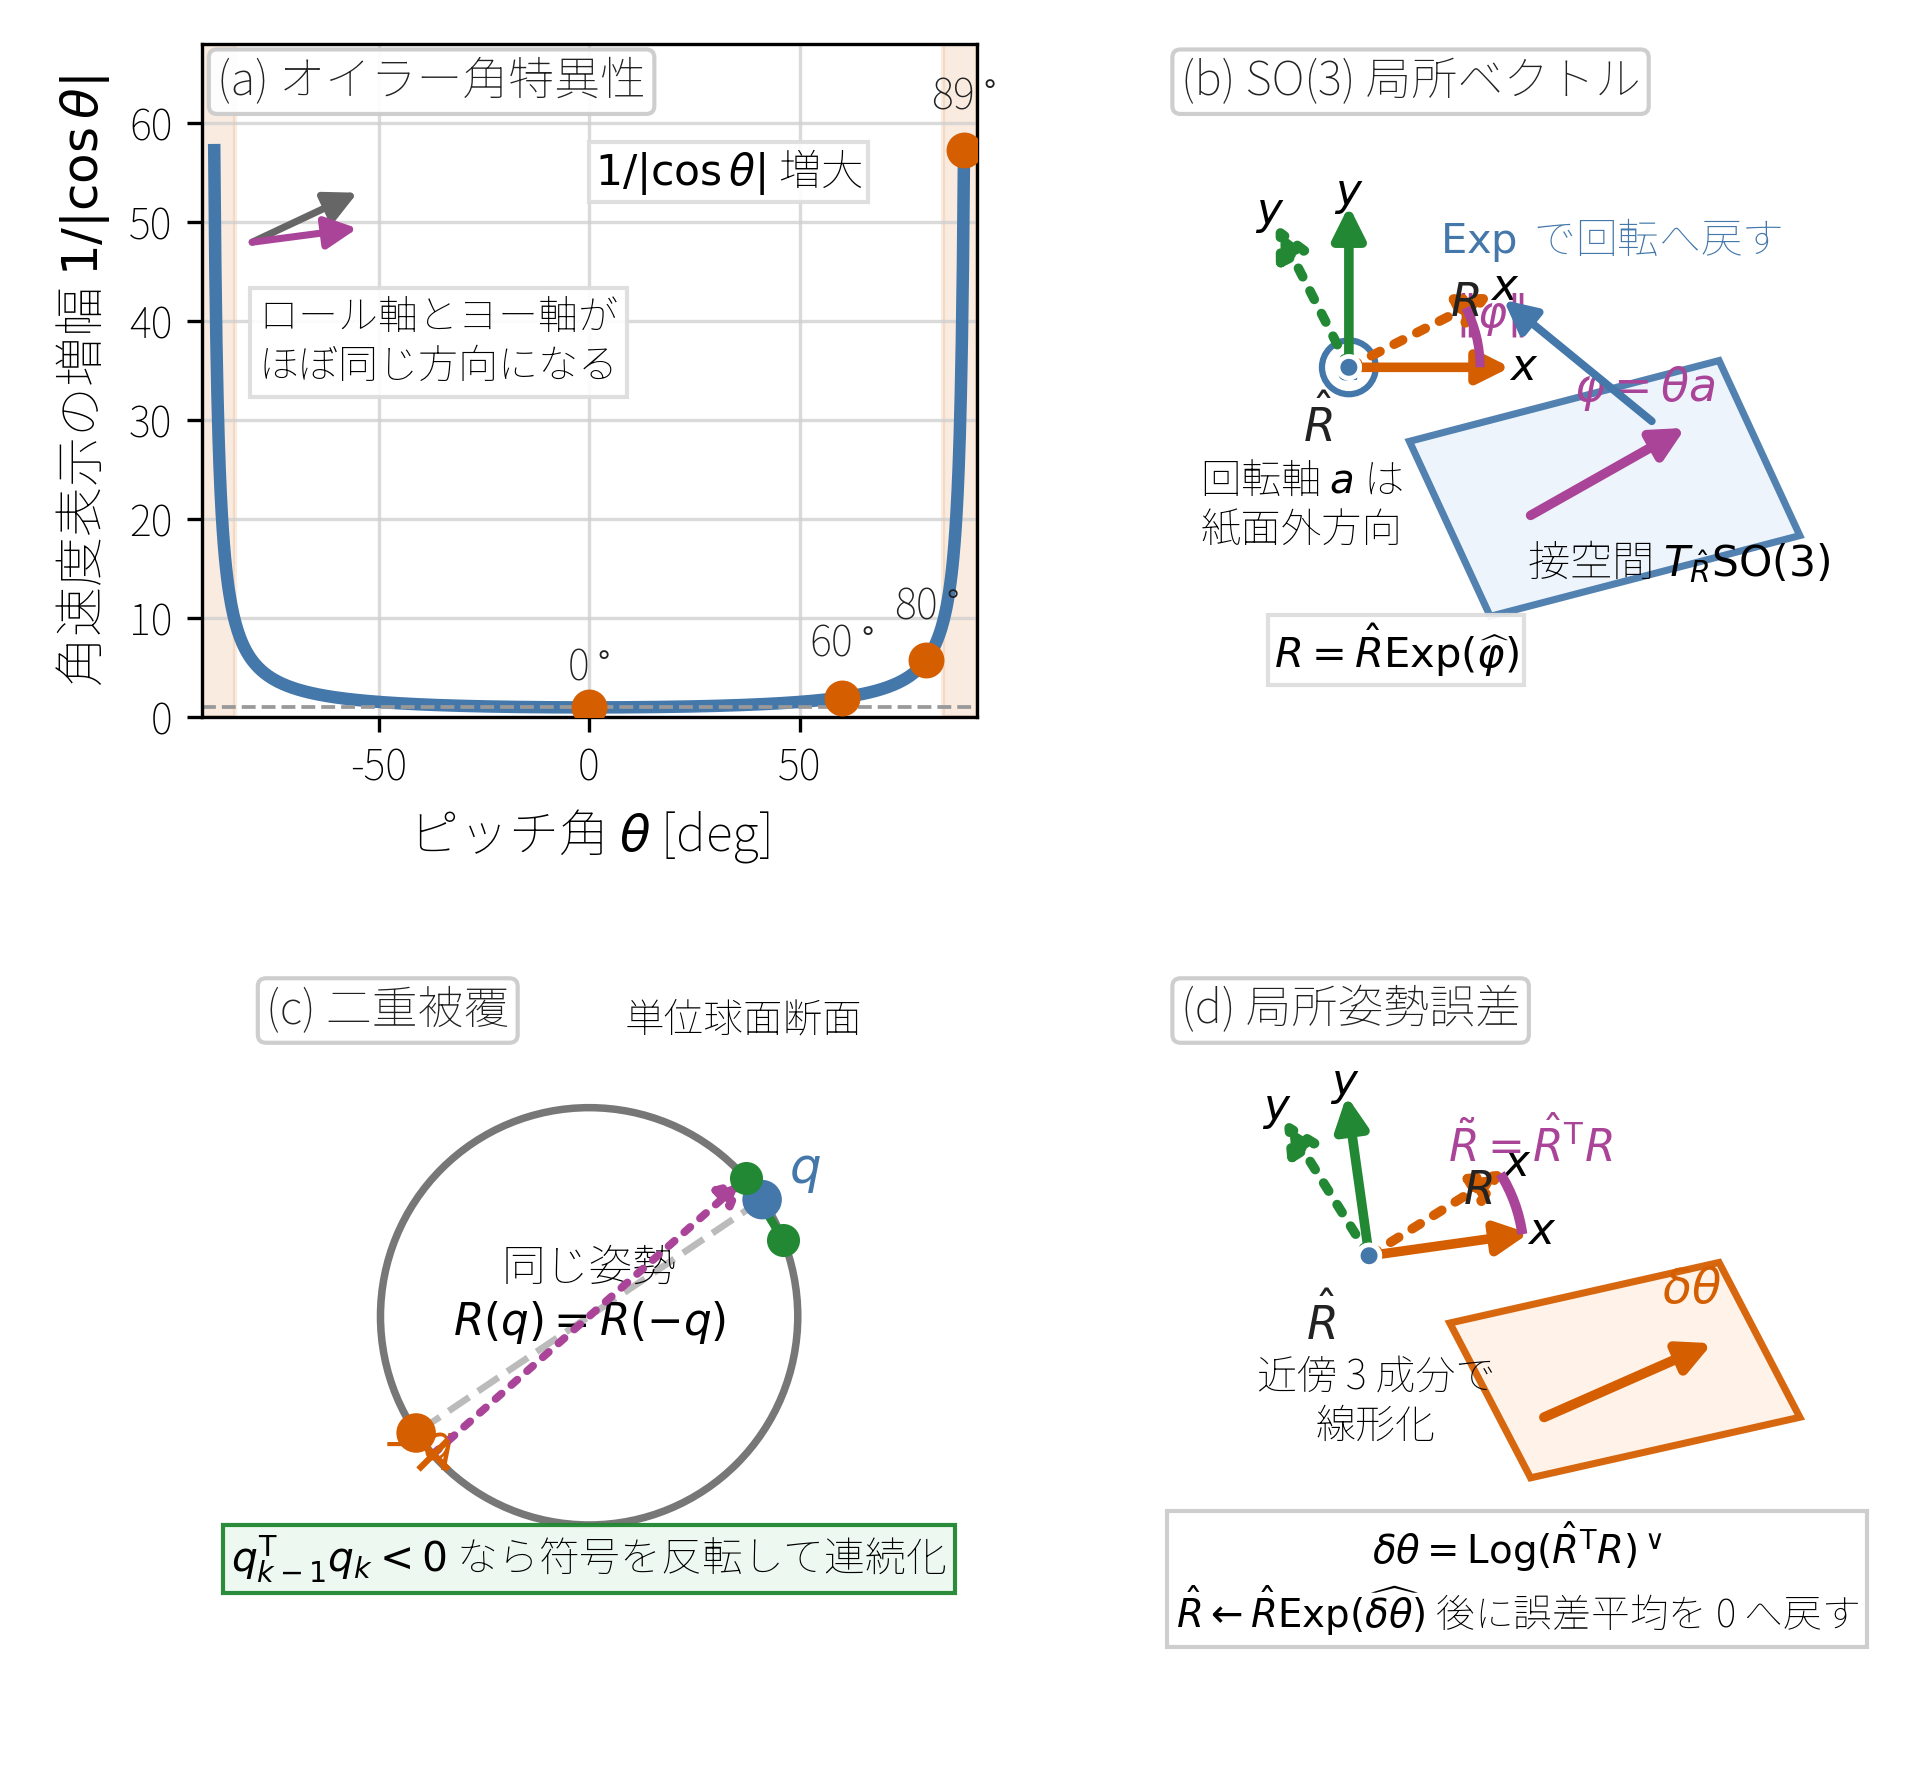
\includegraphics[width=\textwidth]{figures/flow6_attitude_geometry_examples.png}
\caption{三次元姿勢で同時に現れる幾何の要点。オイラー角はピッチ角が $\pm90^\circ$ に近づくと角速度表示が悪条件になり、$\SO(3)$ の指数写像と対数写像は名目姿勢の近くの小回転を接空間で扱う。単位四元数では $q$ と $-q$ が同じ姿勢を表すため、時系列では符号連続性を保つ。ESKF と姿勢制御では、相対回転から局所誤差 $\delta\theta$ を取り出して名目姿勢へ注入する。}
\label{fig:flow-six-attitude-geometry-examples}
\end{figure}

図\ref{fig:flow-six-attitude-geometry-examples}は、この節で導いた式を実装時の判断へ結びつける。左上の曲線は、ZYX オイラー角の逆変換に現れる $1/|\cos\theta|$ をピッチ角で変化させたものである。$\theta=0^\circ$ では機体系角速度 $r=0.10$ [rad/s] がヨー角速度 $\dot{\psi}=0.10$ [rad/s] として表れるが、$\theta=89^\circ$ では同じ実角速度が約 $5.73$ [rad/s] の表示になる。これは剛体が急に速く回ったという意味ではなく、ロール軸とヨー軸が表示上ほぼ同じ方向になり、角度座標が小さな回転を大きな角速度成分へ写すという意味である。

右上の図は、姿勢そのものを $\SO(3)$ 上の点として保ち、小さな回転だけを接空間のベクトル $\varphi$ として扱う見方を表している。$\operatorname{Exp}(\widehat{\varphi})$ は接空間の局所ベクトルを回転へ戻し、$\operatorname{Log}(R)^\vee$ は名目姿勢の近くの相対回転を三次元ベクトルへ戻す。このため、姿勢推定や NMPC の線形化では、全姿勢を一つのオイラー角座標で覆うのではなく、現在の名目姿勢を基準にして「近くの差」だけを線形モデルへ渡す。

左下の四元数の図は、単位四元数の符号が姿勢の符号ではないことを示している。$q$ と $-q$ は同じ回転を表すので、ログ上で符号が飛んでも実姿勢が $180^\circ$ 回ったとは限らない。連続した推定列や補間では、隣り合う四元数の内積が負になったときに片方の符号を反転し、同じ姿勢を近い点として扱う。この処理を入れないと、滑らかな姿勢変化を不連続な誤差として対数写像や補間へ渡してしまう。

右下の図は、ESKF と局所姿勢制御で使う誤差の作り方をまとめている。行列成分を直接引くのではなく、相対回転
\begin{equation}
  \tilde{R}=\hat{R}^\T R
\end{equation}
を作り、
\begin{equation}
  \delta\theta=\operatorname{Log}(\tilde{R})^\vee
\end{equation}
として [rad] 単位の三次元ベクトルを得る。小さい誤差であれば、この $\delta\theta$ は共分散、Kalman ゲイン、フィードバックトルクに入れられる局所座標である。更新後は $\hat{R}\leftarrow\hat{R}\operatorname{Exp}(\widehat{\delta\theta})$ のように名目姿勢へ注入し、誤差平均を 0 に戻す。したがって実装上の帰結は明確である。表示や仕様にはオイラー角を使ってよいが、積分、推定、フィードバック、制約評価では四元数または回転行列で姿勢を保ち、補正量だけを局所ベクトルとして扱う。

姿勢制御でも同じ構造を使う。目標姿勢を $R_d$、現在姿勢を $R$ とすれば
\begin{equation}
  e_R=\operatorname{Log}(R_d^\T R)^\vee
\end{equation}
は、目標姿勢から現在姿勢への局所的な姿勢誤差を [rad] 単位の三次元ベクトルとして与える。角速度誤差 $e_\omega=\omega-\omega_d$ と合わせて
\begin{equation}
  \tau=-K_Re_R-K_\omega e_\omega
\end{equation}
のような局所姿勢制御則を構成できる。ただし、これは小角度誤差を前提とする局所制御則であり、$\pi$ [rad] 近傍の姿勢差、入力飽和、慣性テンソルの不確かさを含む場合は、安定領域と制約を別に評価しなければならない。

以上の理由から、オイラー角、四元数、指数写像、対数写像は競合する表現ではなく、用途の異なる表現である。オイラー角は表示と仕様の記述に適し、四元数は特異点のない姿勢積分と合成に適し、指数写像と対数写像は小さな誤差、共分散、フィードバック誤差を三次元ベクトルとして扱うために適している。姿勢を含む非線形推定、NMPC、剛体姿勢制御では、これらを区別して使うことが、座標特異点と単位制約を破らない実装につながる。
